\documentclass[12pt, twocolumn]{article}
\usepackage{amsmath}
\usepackage{amsfonts}
\usepackage{graphicx}
\usepackage{mathtools}
\usepackage{fullpage}
\usepackage{float}
\usepackage{color, soul}

\begin{document}
\title{6.867 Homework 3: Neural Networks}
\maketitle

\section{Approach}
So far we have only discussed machine learning problems in which we have specified the basis functions we intend to use. However, since the optimal basis functions could be complicated and non-intuitive, such as in the case of images, we may want an approach that allows us to learn the basis functions. Such an approach is Artificial Neural Networks(ANN). 

The idea of a neural network replaces the known basis functions with features, $z_j$ which are parametric functions of activations, $a_j$ learned from the input data in the first layer of learning, and then utilize a second layer to learn the relationship of the output data from those selected features. 
\begin{equation}
a_j^{(1)}= \sum_{i=1}^N w_{ji}^{(1)} x_i+w_{j0}^{(1)}
\end{equation}
\begin{equation}
z_j= g(a_j)
\end{equation}

Where $g(x)$ is a nonlinear map of input to $(0,1)$, generally tanh or sigmoid, and $a_j$ is an activiation, which depends on the data, $x_i, \; i=\{1,...N\}$  and learned weights $w_ji^{(1)}$ and bias $w_0^{(1)}$. 

The second layer learns in a similar fashion and can be describe for $K$ output classes and M features in the  hidden layer  is thus 
\begin{equation}
a_k^{(2)}= \sum_{j=1}^M w_jk^{(2)} z_j+w_{k0}^{(2)}
\end{equation}
\begin{equation}
f_k= \tilde{g}(a_k^{(2)})
\end{equation}
 
Where $\tilde{g}(x)$ is the activation function, another nonlinear map, not necessarily the same as $g(x)$ and $f_k$ is really our prediction $h_k(x,w)$. However for this problem, we will consider them equal, both sigmoids, 

\begin{equation}
\tilde{g}(x)= g(x) = \frac{1}{ 1+e^{-x}}
\end{equation}



\subsection{Gradient Calculation}
First of all we will need the error to calculate the gradient to update our weights and features and apply either regular gradient descent or stochastic gradient descent. To do so,  we must first find the gradient of our cost function, $J$ which depends on the loss function $l(w)$ but also applies a regularization of both sets of weights, $w^{(1)}, w^{(2)}$

\begin{equation}
J= l(w) + \lambda ( ||w^{(1)}||^2_F +||w^{(2)}||^2_F)
\end{equation}

Where the norms above are the matrix Frobenius norm and the loss function, $l(w)$ is the  negative log-likelihood given by 

\begin{equation}
\tiny
l(w)= \sum_{i=1}^N \sum_{k=1}^K -y^{(i)}_k \textrm{log}(h_k(x^{(i)}, w)) - (1 -y^{(i)}_k) \textrm{log}(1 -(h_k(x^{(i)}, w))
\end {equation}


Taking the partial differential of the cost with respect to each variable, $w^{(1)},w^{(2)}$ leads to the gradients. For the gradient with respect to the second layer weights 

\begin{align}
\nabla_{w_k^{(2)}} J (w)= \frac{\partial J}{\partial a^{(2)}_{nk}}  (\nabla w_k^{(2)} a_{nk}^{(2)})  +2 \lambda w_k^{(2)} \\
=\frac{\partial J_n}{\partial h_{nk}} (\tilde{q}' (a_{nk}^{(2)}))z_n + \lambda w_k^{(2)}
\end{align}


algebraically we can solve for the partial of the cost with respect to each prediction where  
\begin{equation}
\frac{\partial J_n}{\partial h_{nk}}= -\frac{y_k^{(n)}}{h_k(x^{(n)},w)} + \frac{1- y_k^{(n)}}{1 - h_k(x^{(n)},w)}
\end{equation}

 Introducing a new variable, $\delta_{nk}^{(2)}$, 
\begin{equation}
\delta_{nk}^{(2)}=\frac{\partial J}{\partial a^{(2)}_{nk}} 
\end{equation}


Looking at the partial with respect to the first layer 

\begin{align}
\nabla_{w_j^{(1)}} J (w)= \frac{\partial J}{\partial a^{(1)}_{nj}}  (\nabla w_j^{(1)} a_{nj}^{(1)}) + 2 \lambda w_j^{(1)}  \\
 = \delta_{nj}^{(1)}  x^{(n)}
\end{align}


Introducing a new variable, $\delta_{nj}^{(1)}$, 
\begin{equation}
\delta_{nj}^{(1)} = \sum_{k=1}^K    \delta_{nk}^{(2)} w_{kj}^{(2)} g'(a_{nj}^{(1)})
\end{equation}

\subsubsection{Stochastic Gradient Descent}
To actually compute optimal weights we will utilize stochastic gradient descent which updates the weights with each new data point,

\begin{equation}
w^{(t+1)} = w^{(t)} + \eta_t \nabla_w J(w^{(t)})
\end{equation}

Where $\eta$ is the learning rate of the form 
\begin{equation}
\eta = \frac{ \alpha}{ (\textrm{iter} + \beta)^\gamma}
\end{equation}

where $\beta \leq 100$, $\gamma >.5$ and iter is the iteration number. 


\subsection{Implementation}
We will use the back propagation algorithm to implement the training of our neural network. The back propagation algorithm is the classic method for training multilayer neural nets. It was introduced in the late 1960s, and was adapted for neural nets in the early 1990s. The algorithm consists of two main phases. the \textit{propagation} phase, and the \textit{weight update} phase.

During the propagation phase, data is fed to the input of the ANN and the activations are propagated forward. After this, the error is propagated backward from the output of the ANN, producing a $\delta$ at each neuron which indicates the computed necessary change at each neuron.

In the weight update phase, each neuron updates its weights according to the error gradient at the node.

This is repeated for each data point and corresponding label. After the entire training set has been used in the back propagation algorithm, the neural net is trained for future predictions.

\section{Results}

We tested out neural net implementation on a few different datasets. We started by testing with two toy dataset provided by the staff, and move on to a simplified version of the popular MNIST dataset.

\subsection{ Toy Data Set}

The toy datasets contains three different classes. They were used mostly to work out the kinks in our ANN implementation, before moving on to the more field-standard MNIST dataset.

The first toy dataset is well separated between the classes, so it will not take too much fine tuning to be able to get good results from our ANN. The second dataset has more overlap between the classes, so the ANN will need to be more carefully optimized.

We ran our ANN implementation on the toy data set using a large range of hidden nodes and regularization constants, and cross validated to find the optimal number, using both batch and stochastic gradient descent. 

We varied the learning rate parameters, number of internal nodes and regularization coefficients and found that the learning rate that worked well for  the toy data sets was $\alpha = 1$, $\beta = 50$, and $\gamma = .6$ in the formulation $\eta = (\alpha/(it + \beta))^\gamma$.

Table1 displays the error rate on the first toy set validation, Table2 show error rate on second toy set, varied across a variety of number of hidden nodes and regularization constants.


\begin{center}
\begin{table}
  \begin{tabular}{ | c | c | c | c | c | c | }
    \hline
     $\lambda$ vs. m & $10^{-10}$ & $10^{-5}$ & $10^{-3}$ & $10^{-2}$ & $10^{-1}$ \\ \hline
     $2$ & 99.0 & 99.0 & 99.0 & 91.7 & 68.0 \\ \hline
     $3$ & 99.3 & 99.3 & 99.3 & 99.0 & 67.7 \\ \hline
     $4$ & 99.3 & 99.3 & 99.3 & 99.0 & 67.7 \\ \hline
     $5$ & 99.3 & 99.3 & 99.3 & 99.0 & 67.7 \\
    \hline
  \end{tabular}
  \caption{ Percent correctly classified using SGD for toy data set 1}
  \end{table}
\end{center}

\begin{center}
\begin{table}
  \begin{tabular}{ | c | c | c | c | c | c | }
    \hline
     $\lambda$ vs. m & $10^{-10}$ & $10^{-5}$ & $10^{-3}$ & $10^{-2}$ & $10^{-1}$ \\ \hline
     $2$ & 89.0 & 88.4 & 88.0 & 66.8 & 33.3 \\ \hline
     $3$ & 92.7 & 93.0 & 93.0 & 93.0 & 33.3 \\ \hline
     $4$ & 92.7 & 93.0 & 93.0 & 93.3 & 33.3 \\ \hline
     $5$ & 92.3 & 93.0 & 92.7 & 92.7 & 33.3 \\
    \hline
  \end{tabular}
  \caption{Percent correctly classified using SGD for toy data set 2}
  \end{table}
\end{center}

As expected, the first dataset is separated well, while the second dataset has some persistent errors. with a proper. For the best choice of number of hidden nodes and gradient descent algorithm, we were able to achieve a correct percentage of 99.3\% for toy dataset 1, and 93.3\% for toy dataset 2.

Figures1-3 provide visuals showing the dataset and the neural net's classification for different values of the free parameters.

Figure1 shows the correctly classified data and the output for $\lambda=10^{-1}$ and $m=3$.

\begin{figure}
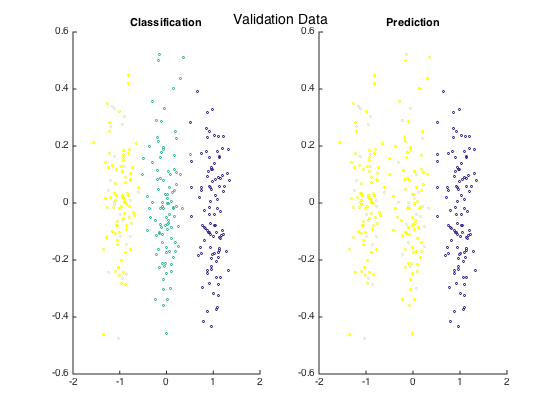
\includegraphics[scale=.4]{toy1val_lambda_min1_m_3.png}
\caption{ Example of result for poorly chosen parameters toy set 1}
\end{figure}

This can be contrasted to what the output classification of figure2 when the parameters are set properly, $\lambda=10^{-10}$ and $m=3$.

\begin{figure}
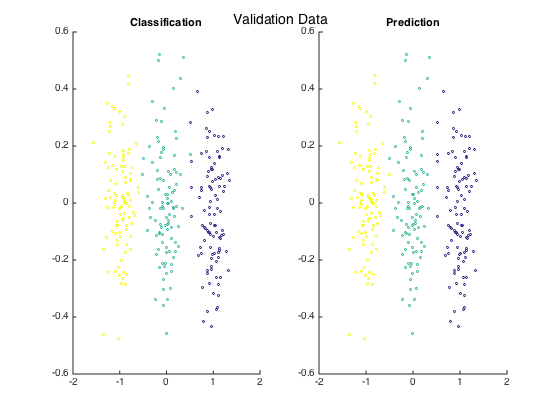
\includegraphics[scale=.4]{toy1val_lambda_min10_m_3.png}
\caption{ Example of result for well chosen parameters for toy set 1}
\end{figure}

It is immediately obvious that better parameters classified the validation set more similarly to the actual classes of the data. 

Finally, figure3 shows the best classification we could get for the second toy dataset with $\lambda=10^{-2}$ and $m=4$.

\begin{figure}
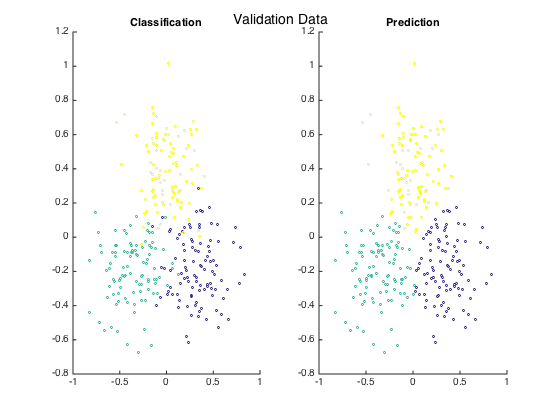
\includegraphics[scale=.4]{toy2val_lambda_min2_m_4.png}
\caption{ well chosen parameters for toy set 2}
\end{figure}

\subsection{MNIST}

The MNIST dataset is a very common dataset in the field of machine learning. It consists of 60,000 training examples, and 10,000 test examples. The inputs are the grayscale pixel values of a 28x28 image of handwritten digits between 0 and 9. The output of the dataset is a vector of length 10, containing nine zeros and one one, indicating the actual number that was written.

This dataset is much more complex than the toy dataset, but still manageable for an ANN. After testing many values for the variety of different free parameters, we were able to achieve a best correct percentage of $92.6\%$. For the learning rate, we used the same formulation, $\eta = (\alpha/(it + \beta))^\gamma$, but this time with $\alpha = .4$, $\beta = 10$, and $\gamma = .55$. Table3 shows values for the free parameters and the corresponding scores they produce.

\begin{center}
\begin{table}
  \begin{tabular}{ | c | c | c | c | }
    \hline
     $\lambda$ vs. m & $10^{-4}$ & $10^{-3}$ & $10^{-2}$ \\ \hline
     $5$ & 17.4 & 90.6 & 89.6 \\ \hline
     $6$ & 17.4 & 92.6 & 90.6 \\ \hline
     $7$ & 17.4 & 92.0 & 90.8 \\ \hline
     $8$ & 17.4 & 91.2 & 91.0 \\ \hline
    \hline
  \end{tabular}
  \caption{Performance of ANN on MNIST dataset for different pairs of $\lambda$ and $m$}
  \end{table}
\end{center}

Something interesting to note is that in this dataset the sensitivity of the parameters in much higher than in the other two toy datasets. This arises because there are so many more data points and the classes have much more overlap. Without the value of the regularization constant being just right, it is very easy to overfit the training data. This causes very bad generalizability, as displayed by table 3. 

In the end, the best choice of parameters proved to be $\lambda = 10^{-3}$, $m=6$, $\alpha = .4$, $\beta = 10$, and $\gamma = .55$ with stochastic gradient descent.

 \end{document}
